\chapter{Arhitektura i dizajn sustava}
		
		\textbf{\textit{dio 1. revizije}}\\
	
	Podsustavi:

\begin{itemize}
    \item Backend (Spring Boot):

\begin{itemize}
        \item Posjeduje više podsustava, uključujući servise i kontrolere za obradu poslovnih zahtjeva.
        \item Spremište podataka temelji se na PostgreSQL bazi podataka, koja je relacijska baza podataka. Relacijske baze omogućuju jednostavan pristup i ažuriranje podataka pomoću tablica koje se sastoje od naziva i niza atributa. Ova struktura omogućuje lako preslikavanje podataka iz aplikacije u bazu i obrnuto.
\end{itemize}

    \item Frontend (Node.js i TypeScript):

\begin{itemize}
        \item Organiziran je u komponente i kontejnere kako bi se omogućilo strukturirano upravljanje korisničkim sučeljem.
        \item Komunicira s backendom putem HTTP protokola, koristeći REST API za razmjenu podataka.
\end{itemize}

\end{itemize}


\begin{itemize}
    \item Baza podataka(PostgreSQL)
\begin{itemize}
    \item omogućuje pouzdanu  pohranu svih relevantnih podataka
    \item  Ova baza podataka služi kao centralno spremište informacija i uključuje niz ključnih tablica i relacija.  
    
\end{itemize}
 

		

				
		\section{Baza podataka}
			
			\textbf{\textit{dio 1. revizije}}\\
			
		\textit{Potrebno je opisati koju vrstu i implementaciju baze podataka ste odabrali, glavne komponente od kojih se sastoji i slično.}
		
			\subsection{Opis tablica}
			

				\textit{Svaku tablicu je potrebno opisati po zadanom predlošku. Lijevo se nalazi točno ime varijable u bazi podataka, u sredini se nalazi tip podataka, a desno se nalazi opis varijable. Svjetlozelenom bojom označite primarni ključ. Svjetlo plavom označite strani ključ}
				
\begin{longtblr}[
    label=none,
    entry=none
]{
    width = \textwidth,
    colspec={|X[6,l]|X[6, l]|X[20, l]|}, 
    rowhead = 1,
}
\hline \SetCell[c=3]{c}{\textbf{ \_user}} \\ \hline[3pt]
\SetCell{LightGreen}id & BIGINT & Jedinstveni identifikator korisnika \\ \hline
active & BOOLEAN & Označava je li korisnik aktivan \\ \hline 
email & VARCHAR & E-mail adresa korisnika \\ \hline 
first\_name & VARCHAR & Ime korisnika \\ \hline 
last\_name & VARCHAR & Prezime korisnika \\ \hline 
password & VARCHAR & Lozinka korisnika \\ \hline 
role & VARCHAR & Rola korisnika (mora biti jedna od predefiniranih uloga) \\ \hline 
\end{longtblr}

				
		
\begin{longtblr}[
    label=none,
    entry=none
]{
    width = \textwidth,
    colspec={|X[6,l]|X[6, l]|X[20, l]|}, 
    rowhead = 1,
}
\hline \SetCell[c=3]{c}{\textbf{imenik}} \\ \hline[3pt]
\SetCell{LightGreen}hlkid & VARCHAR & Jedinstveni identifikator imenika \\ \hline
first\_name & VARCHAR & Ime osobe \\ \hline 
last\_name & VARCHAR & Prezime osobe  \\ \hline 
specialization & VARCHAR & Stručnost osobe  \\ \hline 
active & BOOLEAN & Označava je li osoba u imeniku aktivna \\ \hline 
\end{longtblr}

\begin{longtblr}[
    label=none,
    entry=none
]{
    width = \textwidth,
    colspec={|X[6,l]|X[6, l]|X[20, l]|}, 
    rowhead = 1,
}
\hline \SetCell[c=3]{c}{\textbf{appointment}} \\ \hline[3pt]
\SetCell{LightGreen}id & BIGINT & Jedinstveni identifikator termina \\ \hline 
date\_time & TIMESTAMP & Datum i vrijeme termina \\ \hline
employee\_id & BIGINT & Identifikator zaposlenika koji obavlja termin \\ \hline 
patient\_id & BIGINT & Identifikator pacijenta koji ima termin \\ \hline 
session\_id & BIGINT & Identifikator sesije kojoj pripada termin \\ \hline 
therapy\_id & BIGINT & Identifikator terapije koja se izvodi tijekom termina \\ \hline 
status & VARCHAR & Status termina \\ \hline 
\end{longtblr}

\begin{longtblr}[
    label=none,
    entry=none
]{
    width = \textwidth,
    colspec={|X[6,l]|X[6, l]|X[20, l]|}, 
    rowhead = 1,
}
\hline \SetCell[c=3]{c}{\textbf{employee}} \\ \hline[3pt]
\SetCell{LightGreen}id & BIGINT & Jedinstveni identifikator zaposlenika \\ \hline 
specialization & SMALLINT & Stručnost zaposlenika \\ \hline

\end{longtblr}

\begin{longtblr}[
    label=none,
    entry=none
]{
    width = \textwidth,
    colspec={|X[6,l]|X[6, l]|X[20, l]|}, 
    rowhead = 1,
}
\hline \SetCell[c=3]{c}{\textbf{equipment}} \\ \hline[3pt]
\SetCell{LightGreen}id & BIGINT & Jedinstveni identifikator opreme \\ \hline 
capacity & INTEGER & Kapacitet opreme \\ \hline
description & VARCHAR & Opis opreme \\ \hline 
name & VARCHAR & Naziv opreme \\ \hline 
\end{longtblr}

\begin{longtblr}[
    label=none,
    entry=none
]{
    width = \textwidth,
    colspec={|X[6,l]|X[6, l]|X[20, l]|}, 
    rowhead = 1,
}
\hline \SetCell[c=3]{c}{\textbf{patient}} \\ \hline[3pt]
\SetCell{LightGreen}id & BIGINT & Jedinstveni identifikator pacijenta \\ \hline 
date \_of\_birth & DATE & Datum rođenja pacijenta \\ \hline
address & VARCHAR & Adresa pacijenta \\ \hline 
mbo & VARCHAR & Matični broj osiguranika pacijenta \\ \hline 
phone\_number & VARCHAR & Broj telefona pacijenta \\ \hline 
\end{longtblr}

				
				
			
			\subsection{Dijagram baze podataka}
				\textit{ U ovom potpoglavlju potrebno je umetnuti dijagram baze podataka. Primarni i strani ključevi moraju biti označeni, a tablice povezane. Bazu podataka je potrebno normalizirati. Podsjetite se kolegija "Baze podataka".}
			\begin{figure}
			    \centering
			    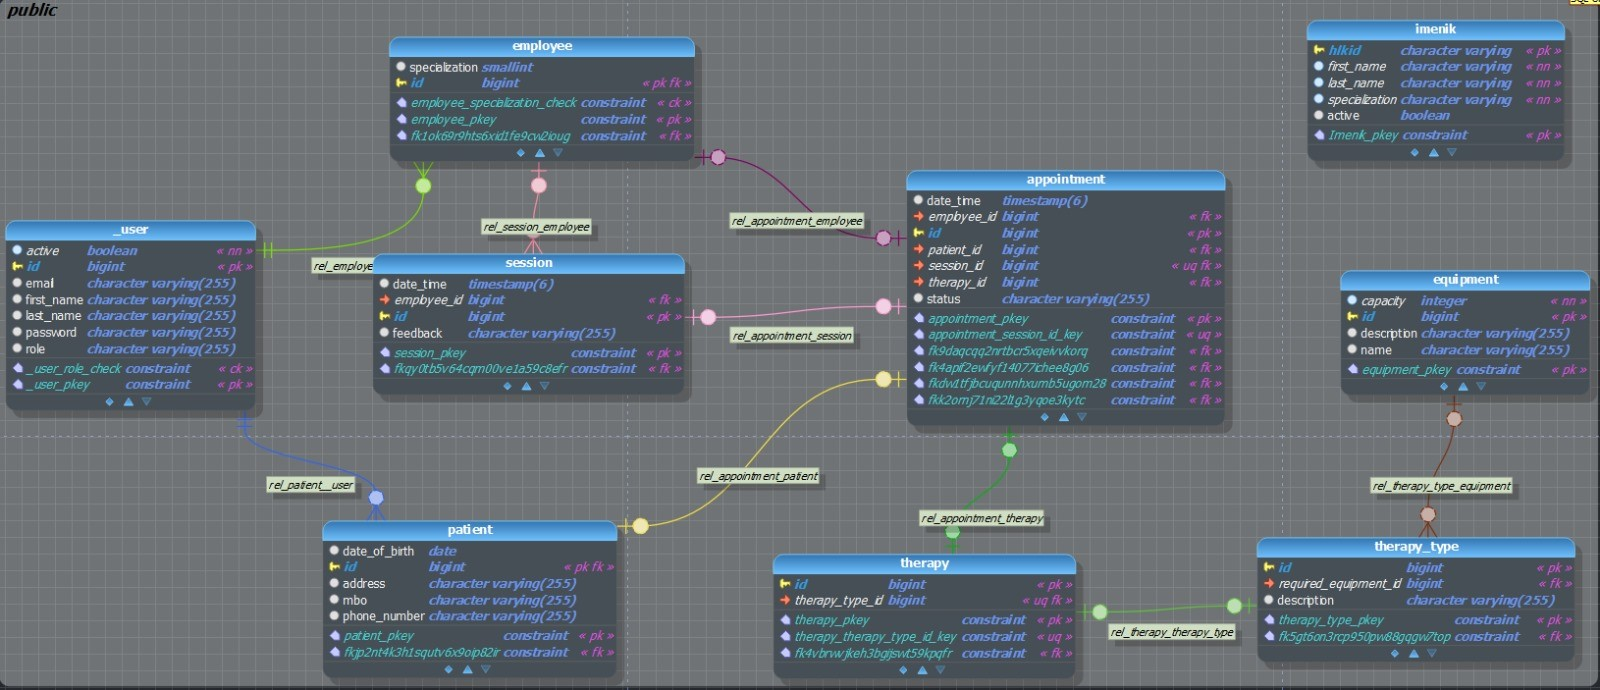
\includegraphics[width=1\linewidth]{database_pr1.jpg}
			    \caption{Dijagram baze podataka}
			    
			    \label{fig:enter-label}
			\end{figure}
			\eject
			
			
		\section{Dijagram razreda}
		
			\textit{Potrebno je priložiti dijagram razreda s pripadajućim opisom. Zbog preglednosti je moguće dijagram razlomiti na više njih, ali moraju biti grupirani prema sličnim razinama apstrakcije i srodnim funkcionalnostima.}\\
			
			\textbf{\textit{dio 1. revizije}}\\
			
			\textit{Prilikom prve predaje projekta, potrebno je priložiti potpuno razrađen dijagram razreda vezan uz \textbf{generičku funkcionalnost} sustava. Ostale funkcionalnosti trebaju biti idejno razrađene u dijagramu sa sljedećim komponentama: nazivi razreda, nazivi metoda i vrste pristupa metodama (npr. javni, zaštićeni), nazivi atributa razreda, veze i odnosi između razreda.}\\
			
			\textbf{\textit{dio 2. revizije}}\\			
			
			\textit{Prilikom druge predaje projekta dijagram razreda i opisi moraju odgovarati stvarnom stanju implementacije}
			
			
			
			\eject
		
		\section{Dijagram stanja}
			
			
			\textbf{\textit{dio 2. revizije}}\\
			
			\textit{Potrebno je priložiti dijagram stanja i opisati ga. Dovoljan je jedan dijagram stanja koji prikazuje \textbf{značajan dio funkcionalnosti} sustava. Na primjer, stanja korisničkog sučelja i tijek korištenja neke ključne funkcionalnosti jesu značajan dio sustava, a registracija i prijava nisu. }
			
			
			\eject 
		
		\section{Dijagram aktivnosti}
			
			\textbf{\textit{dio 2. revizije}}\\
			
			 \textit{Potrebno je priložiti dijagram aktivnosti s pripadajućim opisom. Dijagram aktivnosti treba prikazivati značajan dio sustava.}
			
			\eject
		\section{Dijagram komponenti}
		
			\textbf{\textit{dio 2. revizije}}\\
		
			 \textit{Potrebno je priložiti dijagram komponenti s pripadajućim opisom. Dijagram komponenti treba prikazivati strukturu cijele aplikacije.}